\documentclass[11pt]{article}
\usepackage{setspace}
\setstretch{1}
\usepackage[T1]{fontenc}
\usepackage{amsmath,amssymb, amsthm}
\usepackage{graphicx}
\usepackage{bm}
\usepackage[hang, flushmargin]{footmisc}
\usepackage[colorlinks=true]{hyperref}
\usepackage[nameinlink]{cleveref}
\usepackage{footnotebackref}
\usepackage{url}
\usepackage{listings}
\usepackage[most]{tcolorbox}
\usepackage{inconsolata}
\usepackage[papersize={8.5in,11in}, margin=1in]{geometry}
\usepackage{float}
\usepackage{caption}
\usepackage{esint}
\usepackage{url}
\usepackage{enumitem}
\usepackage{subfig}
\usepackage{wasysym}
\newcommand{\ilc}{\texttt}
\usepackage{etoolbox}
\usepackage{algorithm}
% \usepackage{algorithmic}
\usepackage[noend]{algpseudocode}
\usepackage{tikz}
\usetikzlibrary{matrix,positioning,arrows.meta,arrows}
\patchcmd{\thebibliography}{\section*{\refname}}{}{}{}

\makeatletter
\renewcommand{\@seccntformat}[1]{}
\makeatother


\begin{document}



\title{\textbf{EECS 340: Assignment 7}}

\author{Shaochen (Henry) ZHONG, \ilc{sxz517}}
\date{Due and submitted on 04/27/2020 \\ EECS 340, Dr. Koyut{\"u}rk}
\maketitle

% % % % % % % % % % % % % % % % % % % % % % % % % % % % % % % % % %
% % % % % % % % % % % % % % % % % % % % % % % % % % % % % % % % % %
% % % % % % % % % % % % % % % % % % % % % % % % % % % % % % % % % %
\section{Problem 1}

% % % % % % % % % % % % % % % % % % % % % % % % % % % % % % % % % %
% % % % % % % % % % % % % % % % % % % % % % % % % % % % % % % % % %
\subsection{(a)}

Set the each team as a node (vertex) in graph $G$ and make every node fully connected (representing the fact that all teams have played against each other). If one team $A$ beats another team $B$, we will have a directed edge of $A \rightarrow B$ betwen the nodes representing $A$ and $B$. A team's $z$ is set to be $\infty$ if such team has not won against any other team.

\begin{algorithm}[H]
\caption{DFS-Game-Visit(G, u)}
    \begin{algorithmic}[1]
        \Procedure{DFS-Game-Visit}{G, u}
        \State $z = NULL$ \Comment{Potential $z$ value for this node, if not end of tree.}
        \State $u.color$ = GRAY
        \For{each $v \in Adj(u)$}:
            \If{$v.color$ == WHITE}
                \State $z = v.rank$ \Comment{If have decendent, set decedent's $rank$ as current's $z$.}
                \State $z = \min(z, \textsc{DFS-Game-Visit(G, v)})$ \Comment{Find the lowest $z$ from all decendents.}
            \Else
                \State $z = \min(z, v.z)$ \Comment{Check if explored reachable nodes have lower $z$.}
            \EndIf
        \EndFor
        \State $u.color$ = BLACK
        \If{$z == NULL$} \Comment{If this node is end of tree.}
            \State $u.z = \infty$ \Comment{Set $z$ to $\infty$ to indicate beats no one.}
            \State $z = u.rank$ \Comment{For ancestor nodes to read its rank during recursion.}
        \Else
            \If{$u.z == NULL$}
                \State $u.z = z$
            \Else
                \State $u.z = \min(u.z, z)$ \Comment{If node have been explored, check if the tree's $z$ is better.}
            \EndIf
        \EndIf
        \State \Return $z$
    \end{algorithmic}
\end{algorithm}

\begin{algorithm}[H]
\caption{DFS(G)}
    \begin{algorithmic}[1]
        \Procedure{DFS}{G}
        \For{each $u \in G.V$}:
            \State $u.color$ = WHITE
            \State $u.z = NULL$
        \EndFor
        \For{each $u \in G.V$}:
            \If{$u.color$ == WHITE}
                \State \textsc{DFS-Game-Visit(G, u)}
            \EndIf
        \EndFor
        \For{each $u \in G.V$}:
            \State print $u.team, u.z$ \Comment{output all $z_i$.}
        \EndFor
    \end{algorithmic}
\end{algorithm}



% % % % % % % % % % % % % % % % % % % % % % % % % % % % % % % % % %
% % % % % % % % % % % % % % % % % % % % % % % % % % % % % % % % % %
\subsection{(b)}

\paragraph{Justification for runtime} The algorithm is $O(m+n)$ as DFS will first traverse every node, which means it will at least be $O(n)$. In addition, since the graph $G$ is implemented using adjacency list, for each node we will have to traverse through all its adjacent edges -- where such number can be at most $m$ (total number of edges in $G$) for a single node. Thus, the total time complexity is $O(m + n)$.

\paragraph{Justification for correctness} The algorithm basically performs a DFS travesal on the graph $G$ and set node \ilc{u} with the smallest \ilc{rank} value as \ilc{.z} to all of node \ilc{u}'s ancestor nodes. Due to the nature of DFS, node \ilc{u}'s ancestor nodes can legally have \ilc{u.rank} as their domination factor, as being \ilc{u}'s ancestors imply the fact that these teams have won against team \ilc{u}. Since the graph is implemented as $A$ beats $B$ being $A \rightarrow B$, after the DFS tavesal of a root, all nodes within this DFS tree is guaranteed to have the correct \ilc{.z} value, as all teams have been beaten by these nodes have been checked\footnote{Including \ilc{BLACK} nodes, as shown in \textsc{DFS-Game-Visit}'s \ilc{Line 8-9}: if a node is marked as \ilc{BLACK} it means this node's \ilc{.z} value is correct, so that nodes which are reachable to this \ilc{BLACK} node can simply take its \ilc{.z} value without go into the tree of the \ilc{BLACK} node any further}. \newline
Also in \textsc{DFS-Game-Visit} we will not set a node's \ilc{.z} value unless such node is marked as \ilc{BLACK} (which means all of its decedents have been explored, and all of its reachable node -- regardless marked as \ilc{BLACK} or not, are taken into account). Combine these two observations, each node has explored all of its reachable nodes, and the node's reachable node \ilc{u} with the smallest \ilc{rank} value will be assigned as the \ilc{.z} value of all nodes which have reached node \ilc{u}. The algorithm is a perfect mimic of the game logic of domination factor and guaranteed to be correct.\newline

To speak in a simple way, if we have a node $u$ where $u.rank$ should be the deminate factor of node $x$, we should either have $u$ being a direct decedents of $x$ and therefore promote $u.rank$ as $x.z$ during the DFS travesal from node $x$; or $u$ is explored (marked as \ilc{BLACK}) when $x$ is being traversed, in such case either $u$ or $u$'s ancestor $v$ (marked as \ilc{BLACK} as well) will have the $.z$ value of $u.rank$, and when the travesal of $x$ visits this $u$ or $v$, it will take $u.z$ or $v.z$ directly if it is smaller than its current $z$, and therefore not skiping any beaten team with the lowest \ilc{rank} value. As the algorithm works correctly in both scenarios, the algorithem is guaranteed to be correct.


% % % % % % % % % % % % % % % % % % % % % % % % % % % % % % % % % %
% % % % % % % % % % % % % % % % % % % % % % % % % % % % % % % % % %
% % % % % % % % % % % % % % % % % % % % % % % % % % % % % % % % % %
\section{Problem 2}

Note the tuple below each node represents their \ilc{(start-time, finish-time)}.

\subsection{(a)}

Proof with cases:

There are two possible cases where we can have a $v.f > u.f$:

\begin{itemize}
    \item Case 1: $v.d < u.d < u.f < v.f$\newline
    In this case $u$ is a decent of $v$, which means there must be a path of $v \rightarrow u$; and known that we have $uv \in E$ (from the question instruction), this implies there is a direct connection of $u \rightarrow v$. Thus, now we have a path of $v \rightarrow u$ and a path of $u \rightarrow v$, $uv$ is guaranteed to be on a circle.
    \item Case 2: $u.d < u.f < v.d < v.f$\newline
    In this case we have $u$ completely discovered before $v$. This suggests there shoule be no relationship between $u$ and $v$, as $v$ should not be a decendent nor ancestor of $u$. However, it is known from the question that we have $uv \in E$, which implies $v$ must be a decendent of $u$. Thus, this case will not be valid under the question restriction and therefore disregarded.
\end{itemize}

As all legal case(s) shows $uv$ is guaranteed to be on a circle, we may prove the statement to be true.

\subsection{(b)}

Disprove with conterexample:

\begin{figure}[H]
    \centering
    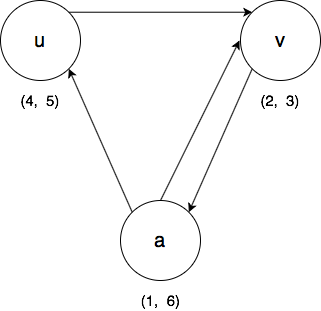
\includegraphics[width=0.35\linewidth]{{fig/fig_2_b.png}}
\end{figure}

It is shown that there is a path from $v$ to $u$ as $v \rightarrow a \rightarrow u$, however $uv$ is still a cross edge as $v.d < v.f < u.d < u.f$ ($2 < 3 < 4 < 5$). Thus, this conterexample disproves the statement.

% % % % % % % % % % % % % % % % % % % % % % % % % % % % % % % % % %
% % % % % % % % % % % % % % % % % % % % % % % % % % % % % % % % % %
% % % % % % % % % % % % % % % % % % % % % % % % % % % % % % % % % %
\section{Problem 4}


\begin{figure}[H]
    \centering
    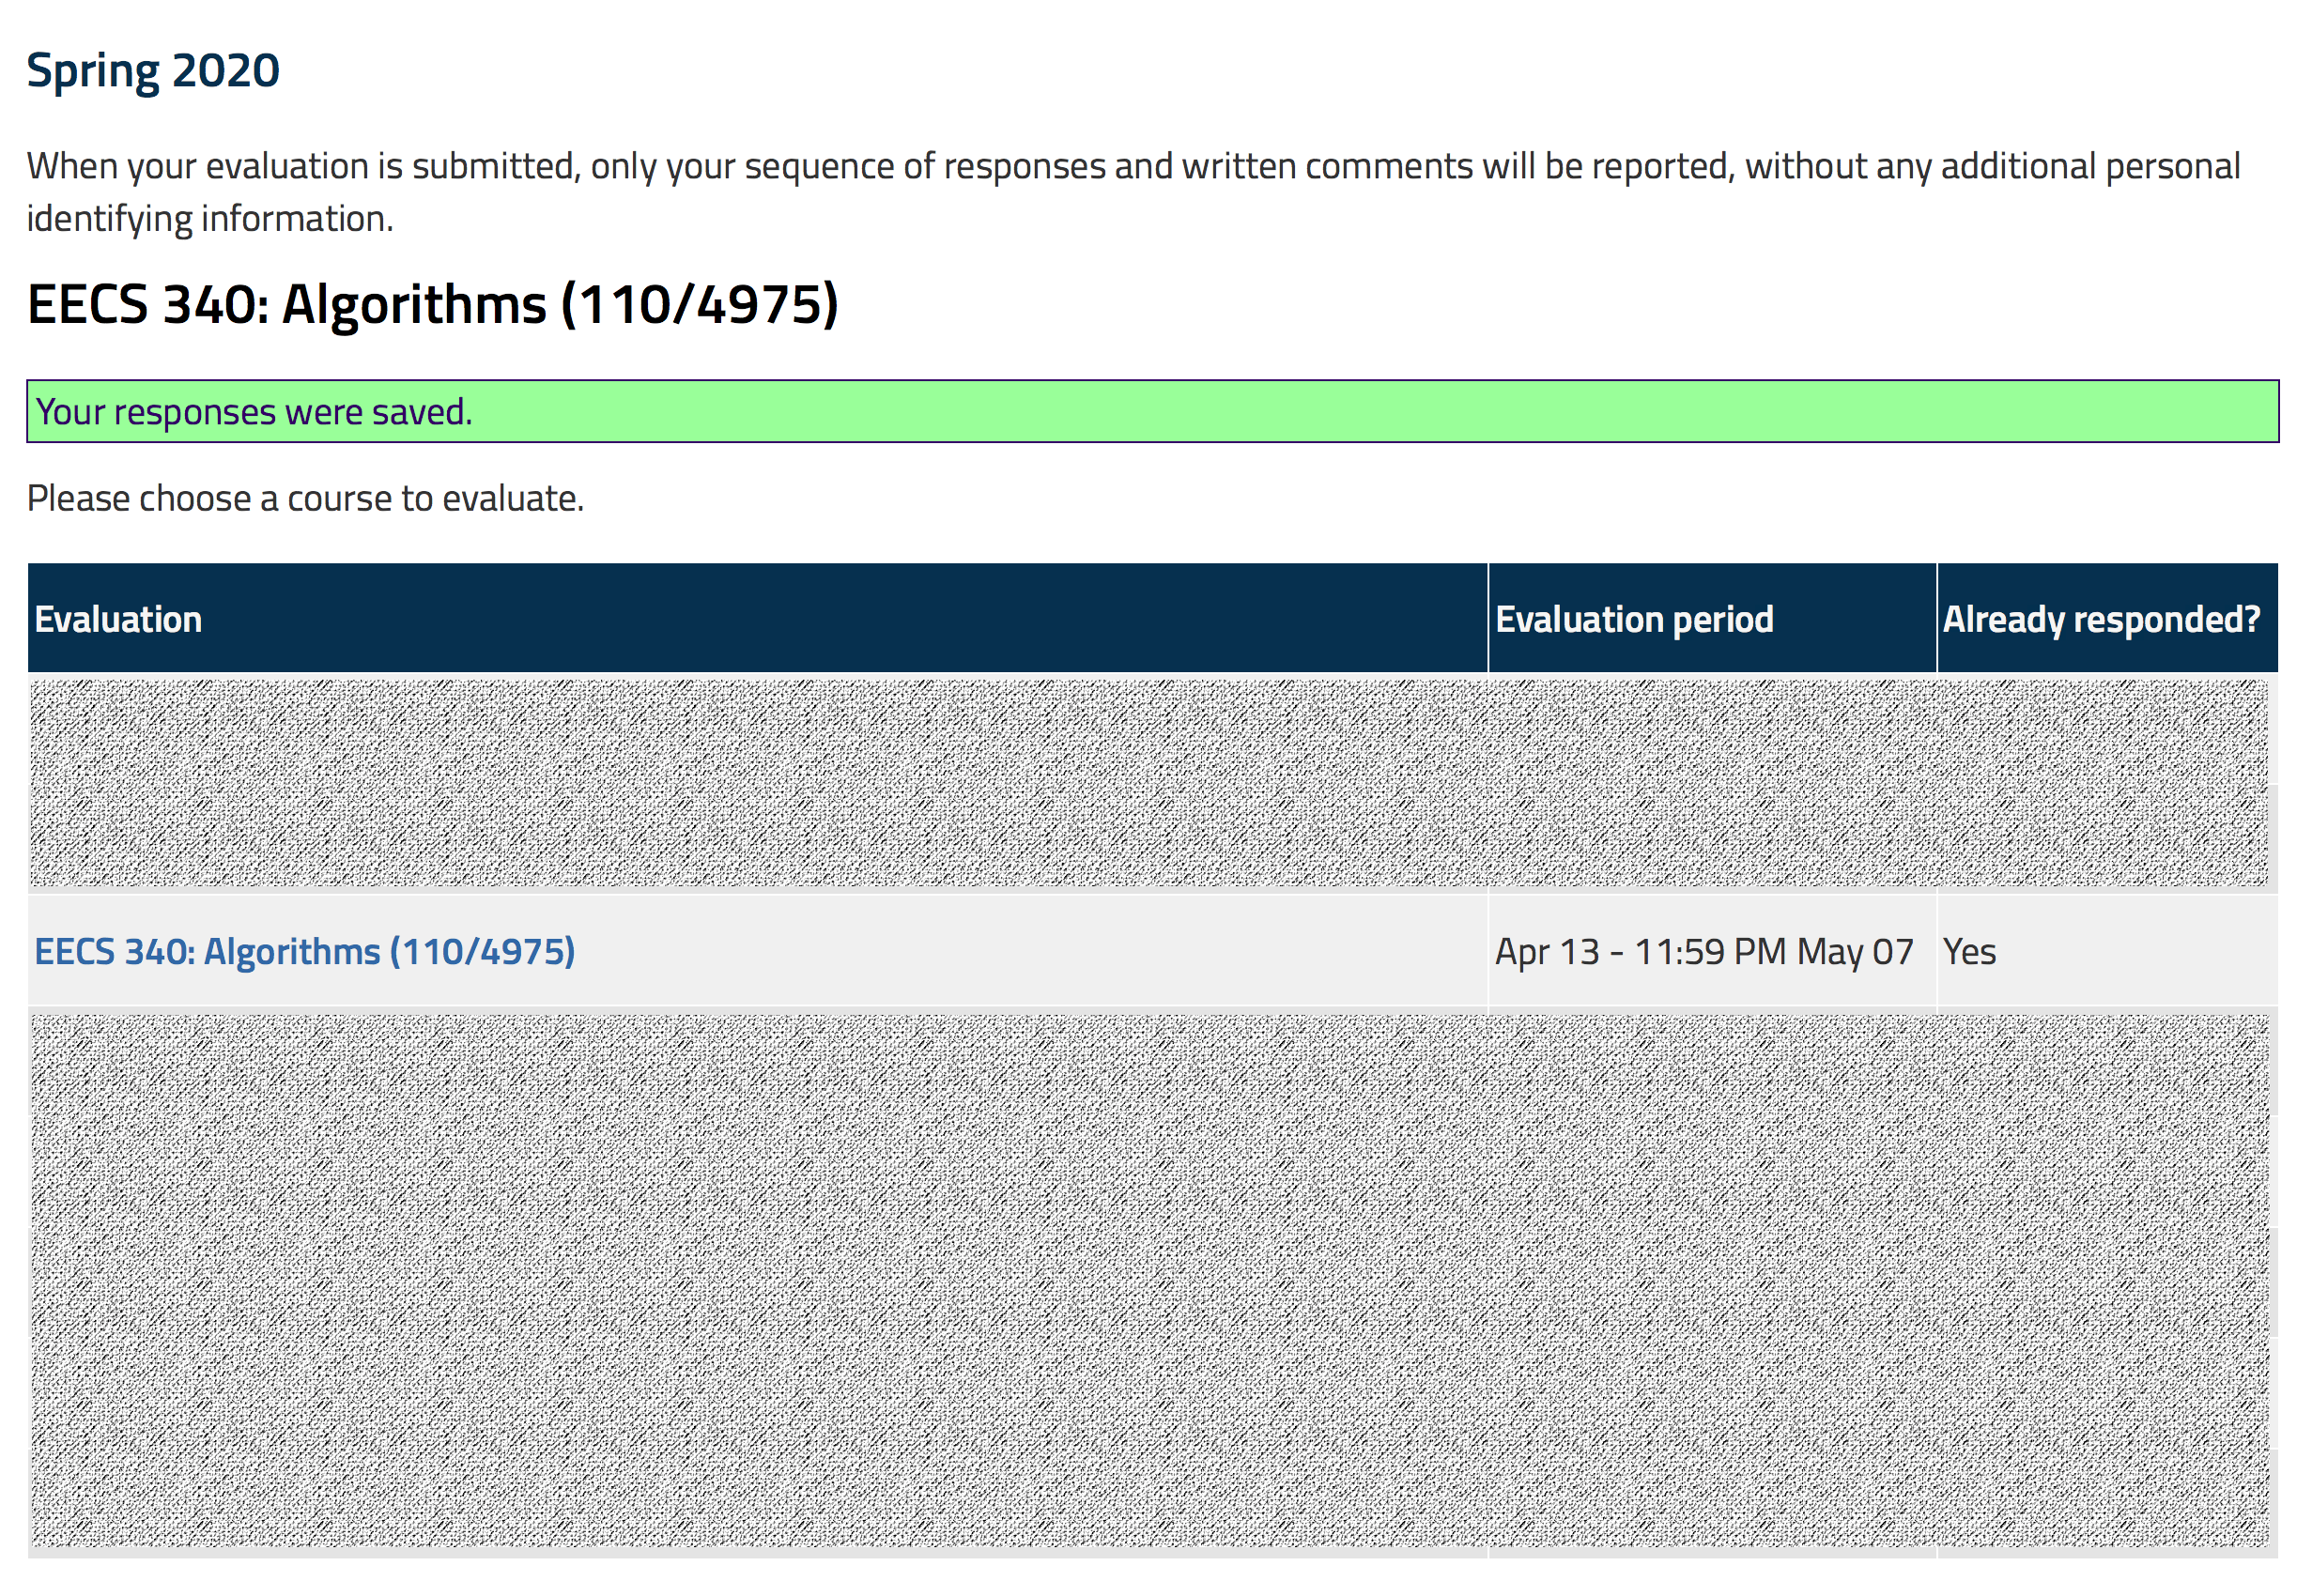
\includegraphics[width=0.7\linewidth]{{fig/fig_4_a.png}}
\end{figure}

% Credit to Peter Grill on https://tex.stackexchange.com/questions/58901/something-between-frownie-and-smiley/59125
\newcommand{\Simley}[1]{%
\begin{tikzpicture}[scale=0.11]
    \newcommand*{\SmileyRadius}{3.0}%
    \draw [fill=brown!10] (0,0) circle (\SmileyRadius)% outside circle
        %node [yshift=-0.22*\SmileyRadius cm] {\tiny #1}% uncomment this to see the smile factor
        ;

    \pgfmathsetmacro{\eyeX}{0.5*\SmileyRadius*cos(30)}
    \pgfmathsetmacro{\eyeY}{0.5*\SmileyRadius*sin(30)}
    \draw [fill=cyan,draw=none] (\eyeX,\eyeY) circle (0.15cm);
    \draw [fill=cyan,draw=none] (-\eyeX,\eyeY) circle (0.15cm);

    \pgfmathsetmacro{\xScale}{2*\eyeX/180}
    \pgfmathsetmacro{\yScale}{1.0*\eyeY}
    \draw[color=red, domain=-\eyeX:\eyeX]
        plot ({\x},{
            -0.1+#1*0.15 % shift the smiley as smile decreases
            -#1*1.75*\yScale*(sin((\x+\eyeX)/\xScale))-\eyeY});
\end{tikzpicture}%
}%

\bigbreak
\bigbreak
\bigbreak

ALL DONE \ \ \Simley{0} \Simley{0.1} \Simley{0.2} \Simley{0.3} \Simley{0.4} \Simley{0.5} \Simley{0.6} \Simley{0.7} \Simley{0.9} \Simley{0.9} \Simley{1} \ \ THANK YOU !!!!!!!!!!!!!!!!!!!!



% \section{References}
%
% \nocite{*}
% \raggedright
% \bibliography{references.bib}
% \bibliographystyle{plain}


\end{document}